\chapter{Superconductivity}
\label{chap:superconductivity}
\section{Calculating $\mu$, $\mu^{*}$}
Since Bogoliubov the screened Coulomb interaction is included in calculations on 
superconductivity assuming it acts like a hard core and 
is ineffective in weakening the phonon-induced attraction.

In Ref.~\cite{morel62} the exact Coulomb interaction is modeled 
as an instantaneous potential, neglecting high-order retarded polarization terms. 
They justify this by saying that dispersion occurs only at rather
high frequencies of the order of the plasma frequency 
and is completely negligible in the small energy range around the Fermi surface.

The instantaneous acting Coulomb interaction is considered 
equivalent to adding a constant to the frequency dependent potential.
%
\begin{equation}
U^{'}(\omega) = \lambda U(\omega) - \mu
\end{equation}
%
Where $\mu$ is the angular average of the Coulomb potential $V(\q)$:
%
\begin{equation}
\mu=\frac{1}{4\pi^{2}v_{0}}\int_{0}^{2k_{0}}\frac{4\pi e^{2}}{k_{s}^{2}+q^{2}}qdq
\end{equation}
%
\begin{equation}
\mu=\frac{k_{s}^{2}}{8k_{0}^{2}}\ln\left[\frac{4k_{0}^{2}+k_{s}^{2}}{k_{s}^{2}}\right]
\end{equation}

$v_{0}$ is the Fermi velocity, $k_{0}$ is the fermi momentum, $k_{s}$ is the screening
wave vector (in a Thomas-Fermi model this would be proportional to the density of states).

If we use the Thomas-Fermi model then: 
%
\begin{equation}
a^{2} = \frac{k^{2}_{s}}{4k^{2}_{0}} = 4\pi e^{2} N_{0}/4k^{2}_{0}
\end{equation}
%
\begin{equation}
\mu = \frac{1}{2} \ln \left[(1+a^{2})/a^{2}\right]
\end{equation}

Just as a note on phonons:
%
\begin{equation}
\lambda = \int_{0}^{1}\left[ \frac{a^{2}}{a^{2} + q^{2}/4k^{2}_{0}}\right]^{2} x dx
\end{equation}
%
where $x=|\k-\k'|/2k_{0}$.

Local fields can be ignored for alkali metals so:
%
\begin{equation}
\lambda \approx \int_{0}^{1} \left[\frac{a^{2}}{a^{2}+x^{2}}\right]^{2}x dx=\frac{1}{2}\frac{a^{2}}{1+a^{2}}
\end{equation}
%
\begin{figure}
\label{fig:supercond}
\begin{center}
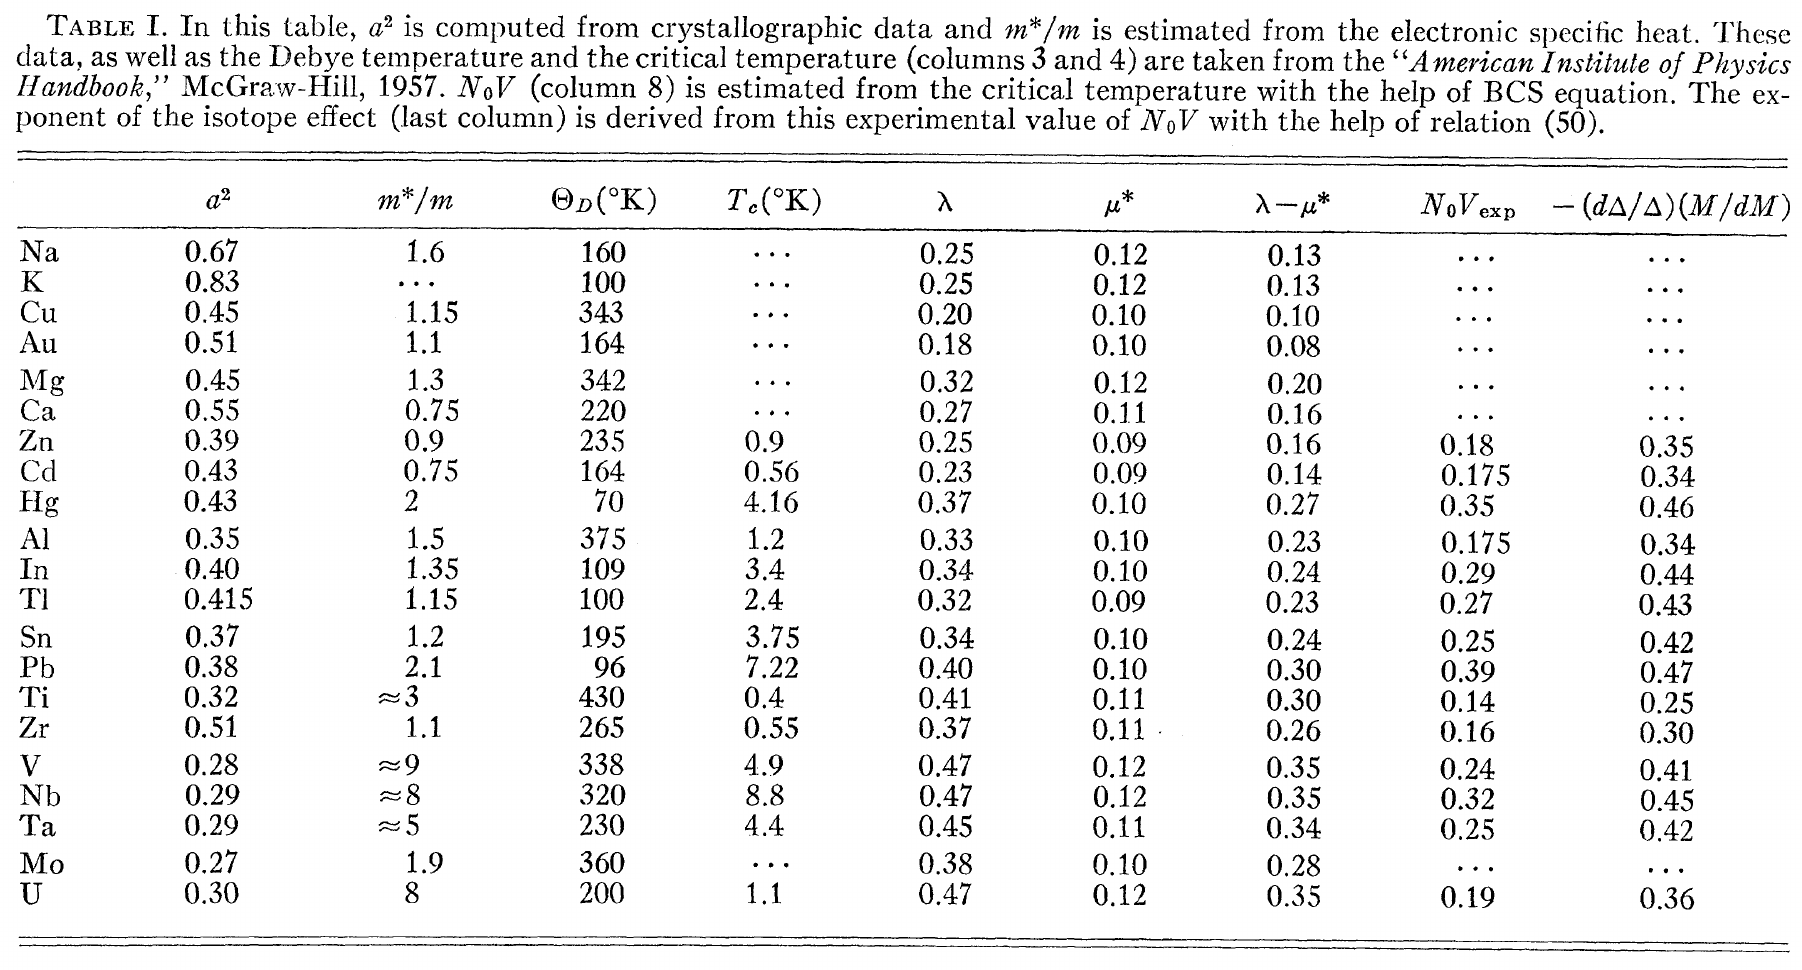
\includegraphics[height=50mm]{./Superconductivity/superconductingparameters.png}
\caption{\small Superconductivity}
\end{center}
\end{figure}
%
When the Coulomb screening is included in the equations for the 
superconducting gap it is modified to be:
%
\begin{equation}
\mu^{*} =  \frac{\mu}{1+ \mu \ln(\frac{\epsilon_{F}}{\theta_{D}})}
\end{equation}
%
\section{Dielectric Matrix Elements}
The above was derived using analytic models in the 60s. Since we have access
to the Fermi surfaces, etc. we can build a more sophisticated model of the
microscopic screening.

The Coulomb repulsion parameter $\mu$ is the Fermi surface average of the Coulomb
scattering matrix elements, $V^{c}_{\k\k'}$:
%
\begin{equation}
\label{eq:fsavg}
\mu = N(0) \bra\bra V^{c}_{\k\k'} \ket\ket_{FS}.
\end{equation}
%

Eq.~\ref{eq:fsavg} can be written explicitly as:
%
\begin{equation}
\mu = \frac{1}{N(0)} \sum_{n\k}\sum_{n'\k'}V^{c}_{n\k,n'\k'}\delta(\epsilon_{n\k}-\epsilon_{F})\delta(\epsilon_{n'\k'}-\epsilon_{F}).
\end{equation}
%

%
\begin{equation}
V^{c}_{n\k,n'\k'} = \bra n'\k'\uparrow, n'-\k'\downarrow |V^{c}| n\k\uparrow, 
n-\k\downarrow\ket
\end{equation}
%
\begin{equation}
V^{c}_{n\k,n'\k'} = \int \psi^{*}_{n'\k'}(\r)\psi^{*}_{n'-\k'}(\r') V^{c}(\r,\r')
\psi_{n\k}(\r)\psi_{n-\k}(\r')\:\rm{d}\r\mathrm{d}\r'
\end{equation}
%

\subsection{Coulomb matrix elements in $\G$ space}
In Ref.~\cite{cohen95} the reciprocal space matrix elements are given.
%
\begin{equation}
\label{eq:cohen1}
V^{c}_{n\k,n'\k'} = \sum_{\G\G'}f^{*}_{n\k,n'\k'}(\G)\epsilon^{-1}(\q+\G,\q+\G')
\times \frac{4\pi e^{2}}{\Omega|\q+\G'|^{2}}f_{n\k,n'\k'}(\G'),
\end{equation}

where $\Omega$ is the crystal volume and $f_{n\k,n'\k'}$ is:
%
\begin{equation}
\label{eq:cohen2}
f_{n\k,n'\k'}(\G) = \sum_{\G'} \psi_{n'\k'}(\G+\G')\psi^{*}_{n\k}(\G')
\end{equation}
%

\subsection{Coulomb matrix elements in SGW}
The convention for two point functions is:
%
\begin{equation}\label{eq.fourier}
 F(\r,\r',\w) = \frac{1}{N_\k\Omega}  \sum_{\k,\G\G'} 
  {\rm e}^{-i(\k+\G)\cdot\r} 
  f_{[\k,\G,\w]}(\G')
  {\rm e}^{i(\k+\G')\cdot\r'}.
\end{equation}
%
The wave function convention for bloch wavefunctions is:
%
\begin{equation}
\psi_{n\k}(\r) = \frac{1}{\sqrt{\Omega}}\sum_{\G}u_{n\k}(\G)e^{i(\k+\G)\cdot\r},
\end{equation}

We have a different sign convention on W so it might be better to rederive
Eqs.~\ref{eq:cohen1} and \ref{eq:cohen2} independently.
%
\begin{equation}
V^{c}_{n\k,n'\k'} = \int \int \psi^{*}_{n'\k'}(\r)\psi_{n\k}(\r)V^{c}(\r,\r')\psi^{*}_{n'-\k'}(\r')\psi_{n-\k}(\r')\rm{d}\r \rm{d}\r'
\end{equation}
%
\begin{equation}
V^{c}(\r,\r') = \frac{1}{N_{\q}\Omega}\sum_{\q,\G,\G'}e^{-i(\q+\G)\cdot\r} \epsilon^{-1}_{\G\G'}(\q,\omega=0)\frac{4\pi e^{2}}{|\q+\G|^{2}} e^{i(\q+\G')\cdot\r'}
\end{equation}
%
First we will do the integral over $\rm{d}\r$ to obtain the constraints on $\q,\G,\G_{1},\G_{2}$:
%
\begin{equation}
V^{c}_{n\k,n'\k'} = \int \int \sum_{\q,\G,\G_{1},\G_{2}} e^{-i(\k'+\q-\k)\cdot\r} e^{-i(\G+\G_{2}-\G_{1})\cdot\r} u^{*}_{n'\k'}(\G) u_{n\k}(\G_{1})\\
\frac{4\pi e^{2}\epsilon^{-1}_{\G_{2}\G_{2}'}}{|\q+\G_{2}|^{2}}...\rm{d}\r\rm{d}\r'.
\end{equation}
%
Then integrating over $\rm{d}\r'$:
%
\begin{multline}
V^{c}_{n\k,n'\k'} = \sum_{\q,\G,\G_{1},\G_{2}} \delta(\k'+\q-\k) \delta(\G+\G_{2}-\G_{1}) u^{*}_{n'\k'}(\G)u_{n\k}(\G_{1})\\
\int \sum_{\G',\G_{1}'\G_{2}'} \frac{4\pi e^{2}\epsilon^{-1}_{\G_{2}\G_{2}'}(\q,\omega=0)}{|\q+\G_{2}|^{2}}
e^{-i(\k-\k'-\q)\cdot\r'} e^{i(\G_{1}'+\G_{2}'-\G')}u^{*}_{n'-\k'}(\G') u_{n-\k}(\G_{1}')\rm{d}\r',
\end{multline}
%
we find:
%
\begin{multline}
V^{c}_{n\k,n'\k'} = \sum_{\q,\G,\G_{1},\G_{2}}\sum_{\G',\G_{1}'\G_{2}'} \delta(\k'+\q-\k)\delta(\G+\G_{2}-\G_{1})\delta(\k-\k'-\q)\delta(\G_{1}'+\G_{2}'-\G')\\ 
u^{*}_{n'\k'}(\G)u_{n\k}(\G_{1})\frac{4\pi e^{2}\epsilon^{-1}_{\G_{2}\G_{2}'}(\q,\omega=0)}{|\q+\G|^{2}} u^{*}_{n'-\k'}(\G')u_{n-\k}(\G_{1}')
\end{multline}

The first constraint on the wave vectors in the brillouin zone is $\q=\k-\k'$. So the change in sign convention
on the dielectric function from Ref.~\cite{cohen95} just means we switch $\k$ and $\k'$. The second
constraint is $\G_{1} = \G + \G_{2}$, and the third constraint is $\G^{'}=\G_{2}+\G_{1}'$. Making
these substitutions we find (multiplying by a $1/\Omega$): 
%
\begin{equation}
V^{c}_{n\k,n'\k'} = \frac{1}{N_{\q}\Omega}\sum_{\G,\G_{2}}\sum_{\G_{1}',\G_{2}'} u^{*}_{n'\k'}(\G)u_{n\k}(\G+\G_{2})
\frac{4\pi e^{2}\epsilon^{-1}_{\G_{2}\G_{2}'}(\q,\omega=0)}{|\q+\G_{2}|^{2}}u^{*}_{n'-\k'}(\G_{1}'+\G_{2}')u_{n-\k}(\G_{1}')
\end{equation}
%
Finally we can introduce the function:
%
\begin{equation}
f_{n'\k',n\k}(\G_{2})= \sum_{\G} u^{*}_{n'\k'}(\G)u_{n\k}(\G+\G_{2})
\end{equation}
%
Or relabeling $\G_{2}=\G$ and $\G=\G'$ we find:
%
\begin{equation}
f_{n'\k',n\k}(\G)= \sum_{\G'} u^{*}_{n'\k'}(\G')u_{n\k}(\G+\G')
\end{equation}
%
If we use time reversal symmetry then we 
recover the expression in Eq.~\ref{eq:cohen2}.
Instead of convolving in $\G$~space it is more convenient to do the products of the
wave functions in real space then apply the dielectric function in $\G$~space:
%
\begin{equation}
f_{n'\k',n\k}(\G) = \int e^{-i(\G\cdot\r)} \psi_{n'\k'}(\r)\psi_{n\k}(\r) \rm{d}\r
\end{equation}
%
Let us resolve $\k'=\k-\q$:
%
\begin{equation}
V^{c}_{n\k,n'\k-\q} = \frac{1}{N_{\q}\Omega}\sum_{\G,\G'}f^{*}_{n'\k-\q,n\k}(\G)
\frac{4\pi e^{2}\epsilon^{-1}_{\G\G'}(\q,\omega=0)}{|\q+\G|^{2}}f_{n'-(\k-\q),n-\k}(\G')
\end{equation}
%
\section{Fermi Surface Average}
Once we are in possession of the matrix elements they must be averaged over the Fermi surface:
%
\begin{equation}
\mu = \frac{1}{N(0)} \sum_{n\k}\sum_{n'\k'}V^{c}_{n\k,n'\k'}\delta(\epsilon_{n\k}-\epsilon_{F})\delta(\epsilon_{n'\k'}-\epsilon_{F}).
\end{equation}
%
$N(0)$ is the density of states per spin at the Fermi energy $\epsilon_{F}$.

The average can be performed using the linear tetrahedron method of Ref.~\cite{lehmann72} or the
the more recent method proposed by Bl\"ochl Ref.~\cite{blochl94}.

\section{Dielectric functions}
\subsection{Lindhard Dielectric Function}
Mahan (may his tribe increase) gives the RPA dielectric function in the static limit:
%
\begin{equation}
\label{eq:statlindhard}
\epsilon(\q,0) = 1 + \frac{q^{2}_{TF}}{2q^{2}}\left[1+\frac{1}{2x}(1-x^{2})\ln\left|\frac{1+x}{1-x}\right|\right]
\end{equation}
%
where $x = q/2k_{F}$.
Eq.~\ref{eq:statlindhard} is what we will use to test our Fermi averaged Coulomb matrix elements.

\subsection{Hubbard Dielectric Function}
The Hubbard dielectric function introduces a correction factor to the RPA of the form:
%
\begin{equation}
\epsilon_{H}(\q,\omega) = 1 - \frac{v_{q}P^{1}(\q,\omega)}{1+ v_{q}G_{H}(\q)P^{1}(\q,\omega)}
\end{equation}
%
where:
%
\begin{equation}
G_{H}(\q) = \frac{1}{2}\frac{q^{2}}{q^{2} + k^{2}_{F}}
\end{equation}
%
Note in atomic units:
%
\begin{equation}
a_{0}q_{TF} = (\frac{4}{\pi}k_{F}a_{0})^{1/2} = \frac{1.5632}{\sqrt{r_{s}}}
\end{equation}
%
and for an electron gas with density $n_{0}$ we find:
%
\begin{equation}
\frac{4\pi n_{0} a^{3}_{0}}{3}r^{3}_{s} = 1
\end{equation}
%
also: 
%
\begin{equation}
n_{0} = \frac{k^{3}_{F}}{3\pi^{2}}
\end{equation}

\section{DFPT}
As nice as model dielectric functions are we would like to construct the
response functions from first principles. To do this we require the full
dielectric matrix as obtained from the Sternheimer method. This requires
the generalization to metals of the DFPT. We follow the treatment given in
the RMP Ref.~\cite{baroni01} and Ref.~\cite{degironcoli95}.

Ref.~\cite{degironcoli95} describes how the (Gaussian) smearing 
technique developed in Refs.~\cite{fu83, methfessel89}.
The tetrahedron method has been employed by Savrasov \cite{savrasov92}.

In the smearing approach the local density of states is convolved 
with a smearing function:
%
\begin{equation}
f(\epsilon)=\frac{1}{\sigma}\tilde{\delta}(\frac{\epsilon}{\sigma}),
\end{equation}
%
which is an approximation to the Dirac $\delta$ function. There
are a variety broadenings which can be chosen: Fermi-Dirac broadening, 
Lorentzian, Gaussian, or Gaussians combined with polynomials.

After the convolution the modified local density of states can be computed accurately on a discrete
grid of k points so long as the energy separation between neighbouring k-points is 
small compared to $\sigma$:
%
\begin{equation}
\label{eq:ldos}
n(\r,\epsilon) = \sum_{i} \frac{1}{\sigma} \tilde{\delta}(\frac{\epsilon-\epsilon_{i}}{\sigma})|\phi_{i}(\r)|^{2}
\end{equation}
%
where $i$ runs over $\k$-points and bands.

The electronic density then follows:
%
\begin{equation}
n(\r)=\int_{-\infty}^{\epsilon_{F}}n(\r,\epsilon)d\epsilon=\sum_{i}\tilde{\theta}(\frac{\epsilon_{F}-\epsilon_{i}}{\sigma})|\phi_{i}(\r)|^{2}
\end{equation}
%
where $\tilde{\theta}(x) = \int_{-\infty}^{x}\tilde{\delta}(y) dy$ is a smooth
approximation to the step function.
%
\begin{equation}
N = \int_{-\infty}^{\epsilon_{F}}n(\epsilon) d\epsilon = \sum_{i} \tilde{\theta}(\frac{\epsilon_{F}- \epsilon_{i}}{\sigma})
\end{equation}
%

Given the definition of Eq.~\ref{eq:ldos} the Kohn-Sham 
kinetic energy functional is given through
the single-particle energy integral:
%
\begin{equation}
T_{s}[n] = \int_{-\infty}^{\epsilon_{F}}\epsilon n(\epsilon)\rm{d}\epsilon-\int V^{KS}(\r)n(\r)d\r
\end{equation}
%
\begin{equation}
T_{s}[n] = \sum_{i} \left[ -\frac{\hbar^{2}}{2m} \tilde{\theta}(\frac{\epsilon_{F}-\epsilon_{i}}{\sigma}) \bra\phi_{i}|\nabla^{2}|\phi_{i}\ket 
+ \sigma\tilde{\theta}_{1}(\frac{\epsilon_{F}-\epsilon_{i}}{\sigma}) \right]
\end{equation}
%
where $\tilde{\theta}_{1}= \int_{-\infty}^{y}y\tilde{\delta}(y)\rm{d}y$.

\subsection{The Sternheimer Eq. In Metallic Systems}
The connection with the Sternheimer approach to density functional perturbation theory can now
be made:
%
\begin{equation}
\label{eq:metallicstern}
%\frac{\partial n(\r)}{\partial \u_{s}} = 2 \sum_{i,\j} \frac{\tilde{\theta}_{F,i} - \tilde{\theta}_{F,j}}{\epsilon_{i} - \epsilon_{j}}
%\tilde{\theta}_{j,i}\phi^{*}_{i}(\r)\phi_{j}(\r) \bra\phi_{j}|\frac{\partial V^{KS}}{\partial\u_{s}} |\phi_{i}\ket
\Delta n(\r) = 2 \sum_{i,j} \frac{\tilde{\theta}_{F,i} - \tilde{\theta}_{F,j}}{\epsilon_{i} - \epsilon_{j}}
\tilde{\theta}_{j,i}\phi^{*}_{i}(\r)\phi_{j}(\r) \bra\phi_{j}|\Delta V|\phi_{i}\ket
\end{equation}
%
Eq.~\ref{eq:metallicstern} can be rewritten:
%
\begin{equation}
\label{eq:nr}
\frac{\partial n(\r)}{\partial \u_{s}} = 2 \sum_{i,j} \phi^{*}_{i}(\r) \Delta \phi_{i}(\r).
\end{equation}
%
Where: 
%
\begin{equation}
%\left[H + Q - \epsilon_{i}\right]\Delta \phi_{i} = -\left[\tilde{\theta}_{F,i}-P_{i}\right]\frac{\partial V^{KS}}{\partial \u_{s}}|\phi_{i}\ket
\left[H + Q - \epsilon_{i}\right]\Delta \phi_{i} = -\left[\tilde{\theta}_{F,i}-P_{i}\right]\Delta V|\phi_{i}\ket
\end{equation}
%
\begin{equation}
\alpha_{k} = \rm{max}(\epsilon_{F} + 3\sigma -\epsilon_{k},0)
\end{equation}
%
\begin{equation}
Q=\sum_{k}\alpha_{k}|\phi_{k}\ket\bra\phi_{k}|
\end{equation}
%
\begin{equation}
P_{i} = \sum_{j} \beta_{i,j}|\phi_{j}\ket\bra\phi_{j}|
\end{equation}
%
\begin{equation}
\beta_{i,j} = \tilde{\theta}_{F,i}\tilde{\theta}_{i,j} + 
\tilde{\theta}_{F,j}\tilde{\theta}_{j,i} + 
\alpha_{j}\frac{\tilde{\theta}_{F,i}-\tilde{\theta}_{F,j}}{\epsilon_{i}-\epsilon_{j}}\tilde{\theta}_{j,i}
\end{equation}
%
The $\alpha_{k}$ is taken to vanish when $\phi_{k}$ is unoccupied then
also $\beta_{i,j}$ vanishes when any of its indices
refers to unoccupied states.

\subsection{$|\q|$=0 Perturbations}
In a periodic system the $|\q|=0$ perturbation may induce a shift of the Fermi
energy. For phonons. In this case Eq.~\ref{eq:nr} becomes:
%
\begin{equation}
\Delta n(\r) = 2 \sum_{n} \phi_{n}^{*}(\r)\Delta\phi_{n}(\r) + n(\r,\epsilon_{F})\Delta\epsilon_{F}
\end{equation}
%
To determine the shift in the Fermi enery we examine the perturbation in the $\q \rightarrow 0$ limit.
%
\begin{equation}
\Delta V_{SCF}(\q) = \Delta V(\q) + \frac{4\pi e^{2}}{q^{2}}\Delta n(\q) \frac{dv_{xc}}{dn}\Delta n(\q)
\end{equation}

The macroscopic component of the density response is:
%
\begin{equation}
\Delta n(\q) = -n(\epsilon_{F}) \Delta V_{SCF}(\q) + \Delta n^{lf}(\q)
\end{equation}
%
\begin{equation}
\Delta_{SCF}(\q) = -\frac{\Delta n_{ext}(\q) -\Delta n^{lf}(\q)}{n(\epsilon_{F}} + \mathcal{O}(q^{2})
\end{equation}

The charge neutrality condition is thus enforced
by a compensating shift in the Fermi energy:
%
\begin{equation}
\Delta \epsilon_{F}=\frac{\Delta n_{ext}(\q=0)+\int n(\r,\epsilon_{F})\Delta V_{SCF}(\r)d\r}{n(\epsilon_{F})}
\end{equation}

\section{Symmetry Properties}
%
We here denote a symmetry operation:
%
\begin{equation}
  \label{eq:symmoperation}
  \symm\r = \S\r + \v
\end{equation}
%
The symmetry reduction can be derived by starting with a real space formulation:
%
\begin{equation}
\label{eq:vcmatel}
V^{c}_{n\k,n'\k'} = \int \int \psi^{*}_{n'\k'}(\r)\psi_{n\k}(\r)V^{c}(\r,\r')\psi^{*}_{n'-\k'}(\r')\psi_{n-\k}(\r')\rm{d}\r \rm{d}\r'
\end{equation}
%
The screened Coulomb interaction posseses the full symmetry properties of the crystal.
%
\begin{equation}
\label{eq:symmw}
V^{c}\left(\symm\r,\symm\rp;\omega\right) = V^{c}(\r,\rp;\omega)
\end{equation}
%
The wavevectors $\psi_{n\k}(\r)$ transform according to the symmetry of the crystal
with the following relationship:
%
\begin{equation}
\label{eq:wavesymm}
\psi_{n\k}(\S\r) = \sum_{m} D(\S)_{nm} \psi_{m\S^{-1}\k}(\r)
\end{equation}
%
The non-symmetrized screened Coulomb interaction is written:
%
\begin{equation}
V^{c}(\r,\r') = \frac{1}{N_{\q}\Omega}\sum_{\q,\G,\G'}e^{-i(\q+\G)\cdot\r} \epsilon^{-1}_{\G\G'}(\q,\omega=0)\frac{4\pi e^{2}}{|\q+\G|^{2}} e^{i(\q+\G')\cdot\r'}
\end{equation}
%
The symmetrized screened Coulomb interaction can be written:
%
\begin{equation}
\label{eq:symmw2}
V^{c}(\r,\r') = \frac{1}{\Omega}\sum_{\S_{n}}\frac{1}{N_{\rm group}}\sum_{\q\in IBZ}{\rm w_{\q}}e^{-i(\q+\G)\cdot\S\r}\epsilon^{-1}_{\q}(\G,\G';\omega=0)v_{\q+\G}e^{i(\q+\G')\cdot\S\r'}e^{i(\G'-\G)\cdot\v}
\end{equation}
%
The only non-zero matrix elements come from $\k'=\k-\q$.

These relations Eq.~\ref{eq:symmw}-Eq.\ref{eq:symmw2} allow 
us to restrict the calculation of $\epsilon_{\q}$ to the irreducible
Brillouin zone. Eq.~\ref{eq:wavesymm} allows us to 
reduce the requirement for the storage of
wavevectors to the IBZ as well. Resulting in a significant 
saving in memory and computational time.

This is similar to the procedure for constructing 
the density from wavevectors in the irreducible 
Brillouin zone. As a reference from Martin we know:
%
\begin{equation}
\label{eq:symmdens}
n(\r) = \frac{1}{N_{\k}}\sum_{i\k}n_{i\k}(\r) = \frac{1}{N_{\rm group}}\sum_{\mathcal{S}_{n}}\sum_{\k\in IBZ}{\rm w}_{\k}\sum_{i}f(\epsilon_{i\k})n_{i\k}(\mathcal{S}_{n}\r + t_{n})
\end{equation}
%
The symmetrized version can be written:
%
\begin{equation}
\bra\bra V^{c}_{n\k n'\k'}\ket\ket=\sum_{\q\in{\rm IBZ}}\sum_{S}\frac{1}{N_{\rm group}}\frac{1}{\Omega}{\rm w}_{\q}\sum_{\k\in {\rm IBZ}}{\rm w}_{\k}\sum_{\G \G'} f_{n\k n'\k'}(\G)\frac{4\pi e^{2}\epsilon_{\q}^{-1}(\G,\G')}{|\q+\G|^{2}}f_{n\k n'\k'}(\G')
\end{equation}
%
I can go one further and sum over the star of q i.e. in this case only use $\S^{-1}\q \neq \q$:
%
\begin{equation}
\bra \bra V^{c}_{n\k n'\k'} \ket \ket = \sum_{\q\in{\rm IBZ}}\sum_{S\in{\rm Star_{\q}}}\frac{1}{N_{\Gs}}\frac{1}{\Omega}{\rm w}_{\q}\sum_{\k\in {\rm IBZ}}{\rm w}_{\k}\sum_{\G \G'}f_{n\k n'\k'}(\G)\frac{4\pi e^{2}\epsilon_{\q}^{-1}(\G,\G')}{|\q+\G|^{2}}f_{n\k n'\k'}(\G')
\end{equation}
%

\subsection{Total Rotation of a Matrix Element}
Now let us apply a rotation of the crystal of the crystal belonging to $\G_{\q}$ for
an arbitrary $\q$ to Eq.~\ref{eq:vcmatel}:
%
\begin{equation}
V^{c}_{n\k,n'\k'} = \int \int \psi^{*}_{n'\k'}(\S\r)\psi_{n\k}(\S\r)V^{c}(\S\r,\S\r')\psi^{*}_{n'-\k'}(\S\r')\psi_{n-\k}(\S\r')\rm{d}\r \rm{d}\r'
\end{equation}
%
By applying Eq.~\ref{eq:wavesymm} and $\S\q=\q$ we obtain a relationship between 
screened Coulomb matrix elements:
%
\begin{equation}
\label{eq:equivmatel}
V^{c}_{n\k,n'\k'} = V^{c}_{n\k_{1},n'\k'_{1}}
\end{equation}
%
Where $\k_{1}=\S^{-1}\k,\quad \S\in\G_{q}$. This relation is important because it allows us to regenerate
the $\mu_{n\k,n'\k'}$ tensor in the full Brillouin Zone.

Two more useful relationships that can be introduced for analysis are band-dependent 
Coulomb repulsion parameters:
%
\begin{equation}
\mu_{nn'} = \frac{1}{N(0)} \sum_{\k,\k'} \frac{\delta(\epsilon_{n\k}-\epsilon_{F})}{N_{n}}V^{c}_{n\k,n'\k'}\delta(\epsilon_{n'\k'}-\epsilon_{F})
\end{equation}
%
\begin{equation}
N_{nn'} = \frac{1}{N(0)} \sum_{\k,\k'}\frac{\delta(\epsilon_{n\k}-\epsilon_{F})}{N_{n}}
\delta(V^{c}_{n\k,n'\k'}-V) \frac{\delta(\epsilon_{n'\k'}-\epsilon_{F})}{N_{n'}}
\end{equation}

\section{Gap Equation With Coulomb Interaction}
In this section I'd like to first reproduce some the results of Ref.~\cite{morel62} `Calculation
of the Superconducting State Parameters with Retarded Electron-Phonon Interaction.' Of specific interest
in that paper is the form of their proposed solution to the Gor'kov-Eliashberg equations with and without
the inclusion of the Coulomb interaction. The work also discusses the solution when there are a range of phonon
frequencies participating in the electron pairing mechanism, and the isotope effect. My primary interest is
in the Coulomb renormalization factor. I'd then like to generalize the renormalization for when plasmon frequencies
are not on the order of the occupied bandwidth and there is anisotropy.
%
\section{$\mu_{\k}$ tensor}
%
In order to produce isosurface plots we can integrate $\mu_{\k\k'}$ over $\k'$ this
gives the effective Coulomb scattering at a particular $\k$ point due to 
all the electrons in the crystal. I calculate this as:
%
\begin{equation}
\label{eq:muktens}
\mu_{\k} = \frac{1}{N(0)}\sum_{\q nn'}V^{c}_{n\k n'\k-\q}{\rm w}_{\k-\q}\delta(\epsilon_{n\k})\delta(\epsilon_{n\k-\q})
\end{equation}
%
Eq.~\ref{eq:muktens} can then be overlayed on the Fermi sheets. 


\section{Morel and Anderson}
%
The article is especially focused on the time dependence of the interactions rather than the
spatial structure of the electron-electron interaction and the electron-phonon interaction.
%
\begin{quote}
Several physical reasons lead us to the conclusion that the coordinate space dependence
of the interaction potential plays a very subsidiary role whereas its retardation 
in time is indeed of major importance in determining the various cutoff phenomena.
\end{quote}
%

\section{Definitions}
%
\begin{eqnarray}
\label{eq:greens}
G(\k,\omega)=-\frac{\omega + \epsilon_{\k}}{\omega^{2}-\epsilon^{2}_{\k}-\Sigma^{2}(\k,\omega)+i\delta}\nonumber\\
F(\k,\omega) = \frac{\Sigma(\k,\omega)}{\omega^{2}-\epsilon^{2}_{\k}-\Sigma^{2}(\k,\omega)+i\delta}
\end{eqnarray}
%
$\Sigma(\k,\omega)$ is the self-energy corresponding to the processes in which two particles either
merge into the condensed phase or emerge from it.
%
\begin{equation}
\label{eq:selfenergy}
\Sigma(\k,\omega) =\frac{i}{(2\pi)^{4}}\int \Gamma(\k-\k',\omega-\omega')F(\k',\omega')d\k'd\omega'
\end{equation}
%
$\Gamma$ is the combination of all elementary electron-phonon and Coulomb interactions and is restricted to lowest order terms only.
%
\begin{equation}
\label{eq:vertex}
D_{0}(\q,\omega) = \alpha_{\q}\left[ \frac{1}{\omega_{q} -\omega -\eta_{\q}} + \frac{1}{\omega_{q}+\omega-\eta_{q}} \right]= \frac{2\alpha^{2}_{\q}}{\omega_{\q}}u_{\q}(\omega)
\end{equation}
%
For small phonon damping the factor $u_{\q}(\omega)$ can be written:
%
\begin{equation}
u_{\q}(\omega) = P\left[\frac{\omega_{\q}^{2}}{\omega_{\q}^{2}-\omega^{2}}\right] + \frac{i\pi}{2}\omega_{\q}
(\delta(\omega+\omega_{\q}) - \delta(\omega-\omega_{\q}))
\end{equation}
%
and V(\q). The Coulomb interaction is approximated by an instantaneous potential.
%
\begin{quote}
This is perfectly acceptable since dispersion occurs only at rather high frequencies of the order of the plasma frequency and is completely negligible in the small energy range we are considering here.
\end{quote}
%
The mathematical structure of the problem is determined 
by Eqs.~\ref{eq:greens}, \ref{eq:selfenergy}, and,~\ref{eq:vertex}

\section{Gap equation with Phonon interaction}

\begin{equation}
\Sigma(\omega) = \frac{i \lambda}{2\pi} \int_{L}\int_{-\infty}^{\infty}d\epsilon'
\frac{\Sigma(z)}{D^{2}-\epsilon^{2}}U(\omega-z)
\end{equation}

\begin{equation}
D(z) =  \left[z^{2} - \Sigma(z)^{2} \right]^{\frac{1}{2}}
\end{equation}

Closing the contour in the upper half plane.

\begin{equation}
\label{eq:sigw}
\Sigma(\omega) = \lambda \int_{(L)} \frac{\omega_{1}}{2} \left[ \frac{1}{\omega_{1} - z + \omega - i\eta} 
+ \frac{1}{\omega_{1} + z - \omega - i\eta} \right] \frac{\Sigma(z)}{2D(z)} dz
\end{equation}

In the time domain Eq.\ref{eq:sigw} looks like:
%
\begin{equation}
\Sigma(t) = \lambda U(t) C(t) = \lambda U(t) \int_{-\infty}^{\infty}F(\k',t)d\epsilon' 
\end{equation}
%
By saying the $F$ function varies slowly with time we arrived at the approximation:
%
\begin{equation}
\Sigma(t) = \lambda U(t)
\end{equation}

So to solve the system of equations self-consistenly we employ
%
\begin{equation}
\Sigma_{1}(\omega) = \Delta U(\omega)
\end{equation}

\begin{equation}
\Sigma_{2}(\omega) = ...
\end{equation}


\section{Gap equation with Phonon and Static Coulomb}

\section{Nambu Formalism}
The total Hamiltonian is:
%
\begin{equation}
H_{0}'= H_{0} + (H_{\chi} + H_{\phi}) - \mu N
\end{equation}
%

The pairing contribution to the Hamiltonian appears as:
%
\begin{equation}
H_{\phi} = \sum_{\k}(\phi^{*}_{k}\ckp\cmkp  + H.c. )
\end{equation}
%

To reduce the two body operator to a one body operator Nambu introduced the two components spinor.

\begin{equation}
\Psi_{k} = 
\begin{pmatrix}
\ck \\
\cmkp
\end{pmatrix}
\end{equation}
%
With the help of the Pauli matrices:
%
\begin{equation}
\tau_{1} =  
\begin{pmatrix}
0 & 1 \\
1 & 0 \\
\end{pmatrix}
\end{equation}
%
\begin{equation}
\tau_{2} =  
\begin{pmatrix}
0 & -i \\
i & 0  \\
\end{pmatrix}
\end{equation}
%
\begin{equation}
\tau_{3} =  
\begin{pmatrix}
1 & 0  \\
0 & -1 \\
\end{pmatrix}
\end{equation}
%
\begin{equation}
1 =  
\begin{pmatrix}
1 & 0 \\
0 & 1 \\
\end{pmatrix}
\end{equation}
%
\begin{equation}
H'_{0} = \sum_{k} \Psi^{+}_{k}[\epsilon_{\k} \tau_{3} + \phi_{\k}\tau_{1} + \phi_{\k}\tau_{2}]\Psi_{k} + \sum_{\k} \bar{\epsilon}_{\k}
\end{equation}
%
where $\bar{\epsilon} = \epsilon_{\k} + \chi_{\k} - \mu$.

The Green's function is now a matrix which we can define in the time domain as:
%
\begin{equation}
\label{eq:nambugrn}
G_{0\alpha\beta}(p,t) =  i\bra 0 |T[\Psi_{p\alpha}(t)\Psi^{+}_{p\beta}(0) ]|0\ket 
\end{equation}
%
Using the previous definitions for our spinors it can be seen that $G_{011}$ and $G_{022}$ are the Green's
functions for the spin up electrons and spin down holes respectively. And the off diagaonal elements
correspond to adding or subtracting a cooper pair with out creating an excitation.
%
%Given the pairing symmetry maybe you can't directly excite the cooper pair with a standard EM wave?
%

Performing a Fourier transform of  Eq.~\ref{eq:nambugreen} one arrives at:
%
\begin{equation}
G_{0}(p,p_{0}) = \frac{(p_{0}I + \bar{\epsilon}\tau_{3} + \phi_{1}\tau_{1} + \phi_{2}\tau_{2}) e^{-\delta p_{0}\tau_{3}}}
{p_{0}^{2} - \bar{\epsilon}^{2} -\phi_{1}^{2} - \phi_{2}^{2} + i\delta}
\end{equation}
%
I think the exponential in the numerator comes in handy when we want to pair the $K_{\pm}$ 
functions with either $\tau_{3}$ or $\tau_{1}$.

Let's alse (re-)introduce $E_{p} = (\bar{\epsilon}^{2} + \phi_{1}^{2} + \phi_{2}^{2})^{(1/2)}$

%
\begin{align}
\Sigma(\p, p_{0}) =  -i\tau_{3}\int 2\bra \p, \p' | V | \p,\p' \ket {\rm Tr}[\tau_{3} G_{0}(p')] \frac{d^{4}p'}{(2\pi)^{4}} \\
   + i \int \bra \p, \p' | V | \p', \p \ket \tau_{3}G_{0}(p') \tau_{3} \frac{d^{4}p'}{(2\pi)^{4}}  \\
   -(\chi_{p} \tau_{3} +\phi_{p_{1}}\tau_{1} + \phi_{p2}\tau_{2})
\end{align}
%

By using Eq.~\ref{eq:gred}:
%
\begin{align}
\Sigma(\p, p_{0}) =  \tau_{3}\int 2\bra\p,\p'|V|\p,\p'\ket - \bra\p,\p'|V|\p',\p\ket v^{2}_{p'} - \chi_{p} \frac{d^{3}p'}{(2\pi)^{3}}\\
							    + \tau_{1} \int \bra\p',\p|V|\p,\p'\ket \frac{\phi_{1p'}}{2E_{p'}} + \phi_{1}  \frac{d^{3}p}{(2\pi^{3})}
							    + \tau_{2} \int \bra\p',\p|V|\p,\p'\ket \frac{\phi_{2p'}}{2E_{p'}} + \phi_{2}  \frac{d^{3}p}{(2\pi^{3})}
\end{align}

Clearly in more modern notation what we have is Hartree-Fock plus the additional 
exchange correlation effects contained in $\chi$ and then the pairing function $\phi$.
If a ground state calculation is performed to obtain some `optimal' single particle
description $\chi$ should be negligible one can then focus on the pairing function.

The self-consistency requires:
%
\begin{equation}
\label{eq:selfconst}
\Sigma(\p,p_{0}) = 0
\end{equation}
%
Using Eq.~\ref{eq:selfconst} and the linear independence of the Pauli operators.

The most general self-energy function can be written function can then be written:
%
\begin{equation}
\Sigma(p) = [1-Z(p)]p_{0}I + \chi(p)\tau_{3} + \phi(p)\tau_{1} + \phi(p)\tau_{2}
\end{equation}
%
And the dyson's equation in matrix form:
%
\begin{equation}
\G = [\G_0^{-1} - \mathbf{\Sigma}]^{-1}
\end{equation}
%
means:
%
\begin{equation}
\G(p) = \frac{Z(p)p_{0}+\bar{\epsilon}(p)\tau_{3}+\phi(p)\tau_{1}}{[Z(p)p_{0}]^{2} - E(p)^{2} + i\delta}
\end{equation}
%
The humble undressed single particle propagator:
%
\begin{equation}
\G_{0}(p) = \frac{p_{0}I + \epsilon_{p}\tau_{3}}{p^{2}_{0} - \epsilon^{2}_{p} + i\delta}
\end{equation}

A few last notes... The single particle Green's function can be factored:
%
\begin{equation}
G_{011} =  \frac{p_{0} + \bar{\epsilon}_{p}}{p_{0}^{2} - E_{p}^{2} + i\delta} = 
\frac{u_{p}^{2}}{p_{0} - E_{p} + i\delta} + \frac{v_{p}^{2}}{p_{0} + E_{p} - i\delta}
\end{equation}
%
\begin{equation}
u_{p}^{2} = \frac{1}{2}(1 + \frac{\bar{\epsilon}}{E_{p}})
\end{equation}
%
\begin{equation}
v_{p}^{2} = \frac{1}{2}(1 - \frac{\bar{\epsilon}}{E_{p}})
\end{equation}

\subsection{Density Sum rules}
The $t=0$ Green's function is given by:
%
\begin{equation} 
-iG_{0}(\p , t=0) =  -i\int G_{0}(\p,p_{0}) \frac{d p_{0}}{2\pi}
\end{equation}
%
\begin{equation} 
\label{eq:gred}
= \frac{ (E_{p} - \bar{\epsilon}_{p})\tau_{3} - \phi_{1}\tau_{1} - \phi_{2}\tau_{2}}{2E_{p}}
\end{equation}

Given the particle number $N_{0}$ is:
%
\begin{equation}
N_{0} = \sum_{\p} (-i) {\rm Tr}\left[\tau_{3}G_{0}(\p, t=0)\right]
\end{equation}
%
\begin{equation}
\int(1- \frac{\bar{\epsilon_{p}}}{E_{p}})\frac{d^{3}p}{(2\pi)^{3}} 
\equiv 2\int v_{p}^{2}\frac{d^{3}\p}{(2\pi)^{3}} = N_{0}
\end{equation}


\section{Notation}
%
Performing integrals in K space is facilitated with these approximations
and relationships:
%
\begin{equation}
\label{eq:sumtoint}
\sum_{p'} \rightarrow \int \frac{d^{3}p'}{(2\pi)^{3}} 
\approx \frac{m}{(2\pi)^{3}p_{F}}\int d\epsilon_{\p'}q dq d\psi
\end{equation}
%
%
where $q$ is not restricted to the first Brillouin zone, and:
\begin{equation}
m d\epsilon_{\p'} \equiv p'dp'
\end{equation}
%
In Eq.~\ref{eq:sumtoint} they have approximated the 3 dimensional
volume integral as an integration over a surface and an integration
over an energy variable. In an isotropic electron gas this is a fine
approximation however in anisotropic system the substitution becomes
less appropriate.
Morel and Anderson have a footnote discussing this effect in Ref.~\cite{morel62}
where they state:
\begin{quote}
The $\q^{-2}$ dependence of $\Gamma(\q,\omega)$ insures the convergence of the original equation (5).
Replacing the integration over $\k'$ by integration over $\epsilon'$ may, however, introduce an artificial divergence
in the case of an instantaneous interaction. We shall in this case cut off
the energy integration at the Fermi energy.
\end{quote}
%
This is the origin of the cutoff of the Fermi 
energy in the Coulomb pseudopotential. When an 
instantaneous Coulomb interaction is assumed there 
is this artificial divergence introduced in 
the gap equation.
%
\begin{equation}
\label{eq:angavg}
\sin\theta d\theta \approx q(\frac{dq}{p_{F}})
\end{equation}

The single-particle density of states at the Fermi
surface is obtained from the effective mass defined by
Eq.~\ref{eq:angavg}:
%
\begin{equation}
N(0) \equiv \frac{m p_{F}}{2\pi^{2}}
\end{equation}
%
Furthermore they are only considering s-wave superconductivity:
%
\begin{equation}
V(p,p') = \int V(p-p')d\Omega_{p-p'}/4\pi
\end{equation}
%
\subsection{Green's Function in Nambu Gor'Kov Formalism}

The Self-energy is given:
%
\begin{equation}
\label{eq:interaction}
\Sigma(p) = i\int \tau_{3} G(p') \tau_{3} \left[\sum_{\lambda} g^{2}_{pp'}D_{\lambda}(p-p') + V_{c}(p-p') \right] 
\frac{d^{4}p'}{(2\pi)^{4}}
\end{equation}
%
From here on out most of the algebra is meant to reduce Eq.~\ref{eq:interaction} 
to a one dimensional integral equation.

\section{Phonon Contribution to the Selfenergy}
The phonon contribution is written:
%
\begin{equation}
\Sigma^{ph}(p) = i \int \tau_{3} G(p') \tau_{3} \sum_{\lambda} g^{2}_{pp'\lambda} D_{\lambda}(p-p')\frac{d^{4}p'}{(2\pi)^{4}}
\end{equation}
%

We are interested primarily in $\Sigma^{\rm ph}(\mathbf{p},p_{0})$ for energies $p_0 < \omega_{D} << E_{F}$. 
Since the phonon propagator decreases as $1/(p_0 - p'_0)^{2}$ for $|p_0 -p'_0| > \omega_{\p-\p'}$ then
the dominant contribution from the $p_{0}'$ integral comes from energies below $\omega_{c}$ where the cutoff
energy is a few times the debye energy. i.e. the cutoff energy on the integral equation only needs to be 
a few times the high characteristic phonon frequency. This also means that the most important kinetic energy
values will also be below the cutoff energy therefore the phonon self energy is approximated as:
%
\begin{equation}
\Sigma(\p,p_{0}) =  \Sigma(p_{F},p_{0})
\end{equation}
%
The integral is now approximated, (In an intentional analogy with what happened in Sec.~\ref{sec:migdal}):
%
\begin{equation}
\Sigma^{\rm ph}(p) =  \frac{im}{(2\pi)^{3}|\p|}\int_{-\infty}^{\infty} d p'_{0} \int_{-\infty}^{\infty}d \epsilon_{p'}
\frac{\left[Z(p_{0}')p'_{0}I - \phi(p^{'}_{0})\tau_{1} \right]}{\left[ (Z(p_{0}')p_{0}')^{2} - \epsilon_{p'}^{2} -\phi^{2}(p_{0}') + i\delta \right]}\sum_{\lambda}\int_{0}^{2k_{F}}q dq g^{2}_{q\lambda} D_{\lambda}(q,p_{0} - p_{0}')
\end{equation}
%
where the same approximations as in Eq.~\ref{eq:migseq} has been used. They have
also assumed particle-hold symmetry to make the $\tau_{3}$ term disappear. 

\subsection{Performing the Frequency integral}
The integration procedure of Eliashberg is used. $D(p-p')$ is broken up into two parts,
$D^{u}$ which is analytic in the upper half of the $p_{0}'$ plane and $D^{l}$ which
is analytic in the lower half plane.

This follows from the spectral representation:
\begin{equation}
D_{\lambda}(\q,q_{0}) = \int_{-\infty}^{\infty} \frac{B_{\lambda}(\q,\omega)d\omega}{q_{0} - \omega + i\omega\delta}
\end{equation}


For the $D^{u}$ term the piece of the $p_{0}'$ contour originally along the positive real axis is folded
through the upper half-plane back along the negative real axis (see diag. where the cuts represent the singularities
of G). Since $D^{u}$ is analytic in the upper half plane is has no discontinuity across the left G-cut. 
Using the relation:
%
\begin{equation}
G(\p, p_{0} + i\delta) = G^{*}(\p, p_{0}-i\delta)
\end{equation}
%
The deformed contour can be replaced by an integral along the lower side of the 
cut if $G(p)$ is replaced by $G(p)-G^{*}(p) = 2i {\rm Im} G(p)$. So the $D^{u}$
contribution gives:
%
\begin{equation}
\Sigma_{u}^{\rm ph}(p) = \frac{-2m}{(2\pi)^{3}|\p|}\int_{-\infty}^{0} d p'_{0} 
{\rm Im}\left[ \int_{-\infty}^{\infty}d \epsilon_{p'}\frac{\left[Z(p_{0}')p'_{0}I - \phi(p^{'}_{0})\tau_{1} \right]}
{\left[(Z(p_{0}')p_{0}')^{2} - \epsilon_{p'}^{2} - \phi^{2}(p_{0}') + i\delta \right]}\right]
\sum_{\lambda}\int_{0}^{2k_{F}}q dq g^{2}_{q\lambda} D^{u}_{\lambda}(q,p_{0} - p_{0}')
\end{equation}
%
Integrating over $d\epsilon'$:
%
\begin{equation}
\Sigma_{u}^{\rm ph} = \frac{m}{(2\pi)^{2}|\p|}\int_{-\infty}^{0} d p'_{0} 
{\rm Re}\left[\frac{\left[ Zp'_{0}I - \phi'\tau_{1} \right]}
{\left[(Zp_{0}')^{2}-\phi^{2}(p_{0}')\right] ^{1/2}}\right]
\sum_{\lambda}\int_{0}^{2k_{F}}q dq g^{2}_{q\lambda} D^{u}_{\lambda}(q,p_{0} - p_{0}')
\end{equation}
%

The $D^{l}$ contribution is handled in a similar manner by folding the negative real axis
piece around and one finds:
%
\begin{equation}
\Sigma_{l}^{\rm ph} = \frac{m}{(2\pi)^{2}}|\p|\int_{0}^{\infty}dp'_{0} 
{\rm Re}\left[\frac{\left[ Z'p'_{0}I - \phi'\tau_{1} \right]}
{\left[(Z'p_{0}')^{2}-\phi^{'2}\right]^{1/2}}\right]
\sum_{\lambda}\int_{0}^{2k_{F}}q dq g^{2}_{q\lambda} D^{u}_{\lambda}(q,p_{0} - p_{0}')
\end{equation}
%

$Z(p)$ and $\phi(p)$ are both even functions of $p_{0}$ and swapping $p_0$ to $-p_0$
in the $D^{u}$ term for $|\mathbf{p}|\approx p_{F}$: 
%
\begin{equation}
\Sigma^{\rm ph}(p) =  \Sigma_{l}^{ph}(p) + \Sigma_{u}^{ph}(p)
\end{equation}
%
\begin{equation}
\label{eq:phoncont}
\Sigma^{\rm ph}(p) =  N(0) \int_{0}^{\infty} dp'_{0}{\rm Re}\left[\frac{Z'p_{0}' I - \phi'\tau_{1}}{((Z'p'_{0})^{2}-\phi'^{2})^{(1/2)}}\right]
K_{\pm}^{\rm ph}(p_{0}, p_{0}') 
\end{equation}
% 
Where the interaction kernels $K_{+}^{\rm ph}$ and $K^{ph}_{-}$ are defined:
%
\begin{equation}
K_{\pm}^{\rm ph}(p_{0},p_{0}') = \sum_{\lambda} \int_{0}^{2k_{F}}\frac{qdq}{2k_{F}^{2}}
\int_{0}^{\infty}d\omega B_{\lambda}(q,\omega) g^{2}_{q\lambda} 
\left[ \frac{1}{p_{0}'+p_{0} + \omega - i\delta } \pm \frac{1}{p'_{0} -p_{0} + \omega - i\delta} \right]
\end{equation}

Where $K_{-}^{\rm ph}$ is to be used with the $I$ component of and $K_{+}^{\rm ph}$ is to be used with the $\tau_{1}$
component in Eq.~\ref{eq:phoncont}.

\section{Spectral Representations}
\subsection{Phonon Green's Function}
Remembering the spectral representations for $D$
%
\begin{equation}
B_{\lambda}(\q,\omega) = \sum_{m} |\bra m| \psi^{+}_{q\lambda}|0\ket|^{2}\delta(\omega-\omega_{m})
- \sum_{m}|\bra m | \psi_{q\lambda} | 0 \ket | ^{2} \delta(\omega+\omega_{m})
\end{equation}
% 
where $\omega_{m}$ is the excitation energy of the n-particle system.
The time Fourier transfor of the system is:
%
\begin{equation}
D_{\lambda} (\q, q_{0}) = \int_{-\infty}^{\infty} \frac{B_{\lambda}(\q,\omega) d\omega}{q_{0}-\omega + i\omega\delta}
\end{equation}
%

Since B is a real quantity the imaginary part of $D$ is:
%
\begin{equation}
{\rm Im} D_{\lambda(\q,q_{0})} = - \pi B_{\lambda}(\q,q_{0}){\rm sgn} q_{0}
\end{equation}
%
and a dispersion relation holds for D:
%
\begin{equation}
D_{\lambda}(\q,q_{0} = -\frac{1}{\pi} \int_{-\infty}^{\infty} \frac{{\rm Im} D_{\lambda}(\q,\omega) {\rm sgn \omega} d\omega}{q_{0} - \omega + i\omega\delta}
\end{equation}

For a system with inversion symmetry:
%
\begin{equation}
\psi_{\q\lambda}^{+} = \psi_{-\q\lambda}
\end{equation}
%
and we can write:
%
\begin{equation}
D_{\lambda}(\q,q_{0}) = \int_{0}^{\infty}B_{\lambda}(\q,\omega) \frac{2\omega}{q^{2}_{0}-\omega^{2}+i\delta}d\omega
\end{equation}
%

For bare phonons:
%
\begin{equation}
B_{\lambda}(\q,\omega) = \delta(|\omega| - \Omega_{q,\lambda}){\rm sgn} \omega
\end{equation}
%
bare phonon propagator:
%
\begin{equation}
D_{0\lambda} = \frac{2\Omega_{q\lambda}}{q_{0}^{2} - \Omega^{2}_{q\lambda}+i\delta}
\end{equation}

\subsection{Dielectric Spectral Representation}
Similar considerations apply for the electronic dielectric function.
Starting from density fluctuation operator:

\begin{equation}
\frac{V_{c}(\q) - V(q)}{V(q)} = \frac{1}{\kappa(q)}-1
\end{equation}

\begin{equation}
= -iV(q) \int_{\infty}^{\infty} e^{iq_{0}\tau} \bra 0|T[\rho_{-q}(-\tau)\rho_{q}(0)]|0\ket
\end{equation}
%

where:
%
\begin{equation}
F(\q,\omega) = V(q) \sum_{n} |\bra n|\rho_{-q}| 0\ket|^{2}\delta(\omega - \omega_{n0}) \quad \omega>0
\end{equation}
%
(note similarity to sternheimer where we are effective taking these matrix elements of the density fluctuation
operator with single particle states). Taking the imaginary part of $F$ gives the spectral function
for the Bose excitations of the electron gas.

We can study the analytic structure of the dielectric function for fixed $\q$ and different $q_{0}$.
%
\begin{equation}
\frac{1}{\kappa(\q,q_{0})} - 1 = \int_{-\infty}^{+\infty} \frac{F(\q,\omega) d\omega}{q_{0} - \omega + iq_{0}\delta}
\end{equation}
%

For a system with inversion symmetry $F(\q,\omega) = -F(\q, -\omega)$ so:
%
\begin{equation}
\frac{1}{\kappa(\q,q_{0})}-1=\int_{0}^{\infty}F(\q,\omega)\left(\frac{1}{q_{0}-\omega+iq_{0}}\delta-\frac{1}{q_{0}+\omega+iq_{0}\delta}\right) d\omega
\end{equation}
%


\section{Coulomb Contribution}
Here we follow the treatment of the Coulomb pseudopotential in
Ref.~\cite{schrieffertext}, and Appendix A of Ref.~\cite{scalpino66}.

In the discusssion  they account for their treatment
of the Coulomb interaction. Since they are primarily interested
in the structure of $\Sigma(\p,i\omega_{n})$ for $\p~\p_{F}$ 
and for $|\omega_{n}|<E_{F}$. In this range the Coulomb
interaction leads to important screening and renormalization
effects, however it does not lead to interesting
variations of $\Sigma$ in a region $\omega_{D}$ about the Fermi
surface as is evident on dimensional grounds.
Thus, for our purposes the Coulomb interaction serves
mainly to renormalize the bare electron and phonon-energy
spectra and screen the electron phonon interaction.

For the phonon contribution we exploited the fact that the interaction takes the 
form of a narrow lorentzian around the Fermi energy. Then we could constrain the 
integral to $p_0'<\omega_{c}$ in quite a straightforward way. The spatial integral 
could then be performed by switch it to an energy integral. To circumvent this
problem an S-wave pseudopotential is meant to map the effect of the coulomb integration
in the energy range outside of $0,\omega_{c}$ back in to that range. In effect it takes
the form of a static, contact potential, i.e. a scalar. 

\begin{equation}
\Sigma^{c}(p) = i\int\tau_{3}G (p')\tau_{3}V_{c}(p-p') \frac{d^{4}p'}{(2\pi^{4})}
\end{equation}

If we define $\phi^{c}$, $\chi^{c}$ and $(1-Z)^{c}p_{0}$ to be the coefficients
of $\tau_{1}$, $\tau_{3}$, and $I$ respectively, we have:
%
\begin{equation}
\label{eq:phi}
\phi^{c}(p) = -i \int \frac{d^{4}p'}{(2pi)^{4}} \frac{\phi'}{(Z'p_{0}')^{2} -\epsilon^{2} - \phi'^{2}} V^{c}(p-p')
\end{equation}
%
\begin{equation}
\label{eq:chi}
\chi^{c}(p) = i \int \frac{d^{4}p'}{(2pi)^{4}} \frac{\epsilon'}{(Z'p_{0}')^{2} -\epsilon^{2} - \phi'^{2}} V^{c}(p-p')
\end{equation}
%
\begin{equation}
\label{eq:Z}
\left[1 - Z(p)\right]^{c}p_{0} = i \int \frac{d^{4}p'}{(2pi)^{4}} \frac{Z'p_{0}'}{(Z'p_{0}')^{2} -\epsilon^{2} - \phi'^{2}} V^{c}(p-p')
\end{equation}

\emph{$V(p-p')$ is assumed to be independent of $p_0'$ and $p_0$.}

This assumption allows us to set Eq.~\ref{eq:Z} 
to zero (the left hand side)  depends on $p_0$ the right hand side doesn't...).
Also Eq.\ref{eq:chi} is neglected because it only effects the 
band renormalization (effective mass) and shifts the chemical potential.
That leaves only $\phi^{c}$:
%
\begin{equation}
\label{eq:phi1}
\phi^{c} = 2 \int_{\Delta}^{\infty}dp_{0}' \int \frac{d^{3}p'}{(2\pi^{3})} {\rm Im} \left[ \frac{\phi'}{(Z'p_{0}') - \epsilon^{2} -\phi'^{2}} 
\right]V^{c}(p-p')
\end{equation}

This reduction has folded the contour as in Fig. 7-7 and used the fact that $2{\rm Im} G$ is the discontinuity across the G-cut. 

Now introduce the pseudo $U$:
%
\begin{equation}
\label{eq:phipseud}
\phi^{c} = 2 \int_{\Delta}^{\omega_c}dp_{0}' \int \frac{d^{3}p'}{(2\pi^{3})} {\rm Im} \left[ \frac{\phi'}{(Z'p_{0}') - \epsilon^{2} -\phi'^{2}} 
\right]U^{c}(p,p')
\end{equation}
%
For Eq.~\ref{eq:phi1} and Eq.~\ref{eq:phipseud} to agree:
%
\begin{equation}
\label{eq:upseudo}
U_{c}(p,p') = V_{c}(\p-\p') + 2 \int_{\omega_{c}}^{\infty}\frac{dp_{0}''}{2\pi}\int \frac{d^{3}\p''}{(2\pi)^{3}}V_{c}(\p-\p'') {\rm Im}
\left[ \frac{1}{p_{0}''^{2} - E''^{2} +i\delta} \right] U(p'',p')
\end{equation}
%
where we have simplified this equation by using $Z(p) \rightarrow 1$, $\phi(p) \rightarrow \phi^{c}(p)$ which follows from the form 
of $K_{+}^{\rm ph}$ and the integral equation, Eq.~\ref{eq:phoncont}. This means outside the integration 
region the electronic self-energy constitutes the dominant contribution. Also $E(p) = [\epsilon^{2}_{p} + \phi^{2}(p)]^{1/2}$

To estimate the magnitude of U we assume s-wave pairing in the superconductor...
In this case only the spherical average of $V^{c}(p-p')$ enters:
%
\begin{equation}
\frac{1}{2}\int V_{c}(p-p') d\mu \equiv V_{c}(p,p')
\end{equation}
%
where $\mu$ is the cosine between $p$ and $p'$. Eq.~\ref{eq:upseudo} then becomes 
{\color{blue} The minus sign comes from the sense in which the contour integral
is taken. If the contour is proceeding in a anti-clockwise fashion around the pole
we find the relation given in the paper. If the integral is taken in a clockwise 
fashion a negative sign appears. In fact the deformation of the Green's function contour 
results in the integral being taken in a clockwise fashion and the minus sign follows
straightforwardly}:
%
\begin{equation}
\int_{\omega_{c}}^{\infty}\frac{d\omega'}{\pi} {\rm Im} \left(\frac{1}{\omega'^{2} - E^{2}_{p'} + i\delta} \right)= \frac{\Theta(E_{p'} - \omega_{c})}{2E_{p'}} 
\end{equation}
%
\begin{equation}
U_{c}(p,p') = V_{c}(p,p') - \int \frac{d^{3}p''}{(2\pi)^{3}} \Theta(E_{p''} - \omega_{c})V_{c}(p,p'') \frac{1}{2E_{p''}}U_{c}(p'',p')
\end{equation}
%

The physical meaning of the pseudo-potential  is just the equation satisfied by the s-wave part 
of the t-matrix for two patricles scattering in the region outside of $\pm \omega_c$ It is reasonable that
the effective potential to use between particles near
the Fermi surface is given by the sum of all multiple scatterings of 
the particles in the region away from the Fermi surface plus the Born term.

If the $V_{c}(p,p')$ is approximated by:
%
\begin{align}
V(p,p') & =  V_{c}, \quad |\epsilon_{p}|, |\epsilon_{p'}| < \omega_{m} \nonumber \\
        & =  0, \quad {\rm otherwise}
\end{align}
%
where $\omega_{m}$ is of order the Fermi energy one finds:
%
\begin{equation}
U_{c}(p,p') = \frac{V_{c}}{1+N(0)V_{c}\ln(\omega_{m}/\omega_{c})}
\end{equation}
%

If the density of Bloch states is constant (i.e. using the usual trick for doing the integrals over 
the Brillouin zone $d^{3}p = m d\epsilon qdq d\psi$.) Physically this suggests scattering far
away from the Fermi surface lead to a smaller probability for two electrons being withing the range of the 
screened Coulomb potential.

Now the three momentum integral can be performed in Eq.~\ref{eq:phipseud} since the important
part of this integral comes when $U_{c}(p,p')$ is a constant. The reduction goes through as for the 
Phonon part of the self-energy and we find:
%
\begin{equation}
\label{eq:inteq}
\Sigma(p) = N(0) \int_{0}^{\omega_{c}}dp^{'}_{0} {\rm Re} \frac{Z'p_{0}'I + \phi'\tau_{1}}{((Z'p_{0}')^{2} - \phi'^{2})^{1/2}} K_{\pm}(p_{0}, p_{0}')
\end{equation}
%

$K_{+}$ is to be used with the $\tau_{1}$ component and $K_{-}$ with the $I$ component. The Coulomb pseudopotential only contributes
to the $K_{+}$ component. Had the dynamic dielectric function function been used and no particle hole symmetry been assumed the
Coulomb interaction would have entered $K_{-}$ as well (had we not dropped the $[1-Z(p)]^{c}$ term).

%
\begin{equation}
K_{+} (p_{0},p_{0}') = K _{+}^{\rm ph}(p_{0},p_{0}') - U_{c}
\end{equation}

\begin{equation}
K_{-} (p_{0},p_{0}') = K _{-}^{\rm ph}(p_{0},p_{0}') 
\end{equation}

\section{Gap Equations}
%
The integral equation Eq.~\ref{eq:inteq} can be simplified by introducing:
%
\begin{equation}
\Delta(p_{0}) \equiv \frac{\phi(p_{0})}{Z(p_{0})} 
\end{equation}
%
This is basically the BCS energy gap parameter. One then finally obtains:
%
\begin{equation}
\Delta(p_{0}) = \frac{N(0)}{Z(p_{0})} \int_{\Delta_{0}}^{\omega_{c}} d p_{0}' {\rm Re} \left[ 
\frac{\Delta(p_{0})}{(p_{0}'^{2} - \Delta^{2}(p_{0}'))^{1/2}} 
\right]K_{+}(p_{0}, p_{0}') 
\end{equation}
%
and
%
\begin{equation}
\left[ 1-Z(p_{0}) \right] p_{0} = N(0) \int_{\Delta_{0}}^{\omega_{c}}d p_{0}'
{\rm Re} \left[ \frac{p_{0}'}{(p_{0}'^{2} - \Delta^{2}(p_{0}'))^{1/2}}\right]K_{-}
\end{equation}

Finally the famous $\Delta_{0} = \Delta(\Delta_{0})$ defines the gap parameter at the edge
of the gap.

I need to compare this with Roxana's anisotropic paper but a quick glance shows everything looks
fairly straightforward. So then the path becomes put in the Morel Andersen notes so we can switch
to the time domain easily, and do the derivations with a dynamic Coulomb contribution. 

\section{Coulomb Contribution to the Selfenergy}
%
A more detailed derivation of the Coulomb term in the Eliashberg equations
is given in the Scalapino et. al. paper.
%
The Coulomb part of the electronic self-energy is given by:
%
\begin{equation}
\Sigma^{c}(p) = - \int \frac{d^{3}p'}{(2\pi)^{3}}\int_{-\infty}^{\infty}\frac{d\omega'}{2\pi}{\rm Im}[\tau_{3}G(p',\omega')\tau_{3}] V(p,p')\tanh(\beta\omega'/2)
\end{equation}
%
\begin{equation}
\label{eq:phic}
\phi^{c}(p)\equiv \frac{1}{\pi}\int_{0}^{\infty}d\omega'\int\frac{d^{3}p'}{(2\pi)^{3}}
{\rm Im}(\frac{\phi(p',\omega')}{Z^{2}(p',\omega')\omega'^{2} -\epsilon^{2}_{p'}-\phi^{2}(p',\omega')+i\delta})
V(p,p') \tanh(\beta\omega'/2)
\end{equation}
%
The Coulomb pseudopotential effectively maps the energy integration from
$0\rightarrow \infty$ to $0 \rightarrow 10 \omega_{D}$. We will derive $U_{c}$ in
the next section.

Before doing all the derivations we write down the final results. The $p'$ integration in
Eq.~\ref{eq:phic} is performed by exploiting the rapid decrease of $G(p',\omega')$ 
for large $|\epsilon_{p'}|$ (so long as $|\omega'|<\omega_{c}$):
%
\begin{equation}
\phi^{c}(p) \approx \phi^{c}(p_{F})
\end{equation}
%
The quantity entering the Eliashberg formalism is then:
\begin{eqnarray}
\phi^{c}(p_{F}) =  -N(0) \int_{0}^{\omega_{c}}d\omega' {\rm Re}\left(\frac{\phi(\omega')}{(Z^{2}(\omega')\omega'^{2} - \phi^{2}(\omega'))^{1/2}}\right)
\times U_{c} \tanh(\beta\omega'/2).
\end{eqnarray}
%
$U_{c}$ will be recognized more widely as $\mu^{*}$.
%
\section{The Assumptions and Derivation}
%
Firstly Eq.~\ref{eq:phic} is rewritten:
%
\begin{eqnarray}
\label{eq:phic1}
\phi^{c}(p) = \frac{1}{\pi}\left[\int_{0}^{\omega_{c}} d\omega' + \int_{\omega_{c}}^{\infty} d\omega' \right]
\int \frac{d^{3} p'}{(2\pi)^{3}}{\rm Im}\left(\frac{\phi(p',\omega')}
{Z^{2}(p',\omega')\omega'^{2}-\epsilon_{p'}^{2}-\phi^{2}(p',\omega') +i\delta}\right)V(p,p')\tanh(\beta \omega'/2)
\end{eqnarray}
%
Some assumptions:
%
\begin{itemize}
\item $Z(p,\omega) \rightarrow 1$ and $\phi(p,\omega)\rightarrow \phi^{c}(p)$ for $\omega>>\omega_{D}$ since
the electron-phonon interaction is ineffective except for energies $\omega>\omega_{D}$.

\item $\beta\omega_{c}>>1$ for temperatures at which the material is superconducting, so that 
$\tanh(\beta\omega'/2)\approx 1$ for $\omega'>\omega_{c}$. 

\item So $\tanh$ and $Z$ functions are replaced by unity and $\phi(p',\omega)$ 
goes to $\phi^{c}(p)$. (HL: at this stage we could examine $\phi^{c}(p,\omega)$.
\end{itemize}
%
Using these assumptions this simplifies Eq.~\ref{eq:phic} to: 
%
\begin{align}
\label{eq:intphi}
\phi^{c}(p) + \int \frac{d^{3}p'}{(2\pi)^{3}}V(p,p')
\frac{\Theta(E_{p'}-\omega_{c})}{2E_{p'}}\phi^{c}(p') \nonumber & &\\
 = \int \frac{d^{3}p'}{(2\pi)^{3}}V(p,p') & \int_{0}^{\omega_{c}}\frac{d\omega'}{\pi} &
{\rm Im}\left(\frac{\phi(p',\omega')}{Z^{2}(p', \omega')\omega'^{2}-\epsilon^{2}_{p'}-\phi^{2}(p',\omega')}\right)\tanh(\beta\omega'/2)
\end{align}

This reduction has used the relation:
%
\begin{equation}
\label{eq:pair}
\int_{\omega_{c}}^{\infty} \frac{d\omega'}{\pi}{\rm Im} (\frac{1}{\omega'^{2}-E^{2}_{p'}+i\delta}) 
= \frac{\theta(E_{p'}-\omega_{c})}{2E_{p'}}
\end{equation}

Now if we allow the integration over $p$ to be thought of as a matrix summation
Eq.~\ref{eq:intphi} becomes:
%
\begin{equation}
\label{eq:matrixcoul}
(1+\Omega)\phi^{c}=VF
\end{equation}
%
where the matrix elements take the form:
%
\begin{equation}
\Omega_{[pp']} =  \left[\frac{\Theta(E_{p'}-\omega_{c})}{2E_{p'}}\right]V(p-p')
\end{equation}

\begin{equation}
\label{eq:Fp}
F_{p'}= \int_{0}^{\omega_{c}}\frac{d\omega'}{\pi}{\rm Im}\left(\frac{\phi(p',\omega')}{Z^{2}(p',\omega')\omega'^{2}
-\epsilon^{2}_{p'} -\phi^{2}(p',\omega') }\right)\tanh(\beta\omega'/2)
\end{equation}
%
Since V is a repulsive potential, $[1+\Omega]$ is non-singular and Eq.~\ref{eq:matrixcoul}
can be inverted:
\begin{equation}
\label{eq:matphi}
\phi^{c} = [1+\Omega]^{-1}VF \equiv U_{c}F
\end{equation}
%
Where $U_{c}$ satisfies:
%
\begin{equation}
[1+\Omega]U_{c} = V
\end{equation}
%
This means, in component form, $U_c$ can be determined by the integral equation:
%
\begin{equation}
\label{eq:integu}
U_{c}(p,p') = V(p-p') - \int \frac{d^{3}p'}{(2\pi)^{3}}V(p,p'')\times
\frac{\Theta(E_{p''}-\omega_{c})}{2E_{p''}}U_{c}(p'',p')
\end{equation}
%
By taking components of Eq.~\ref{eq:matphi} one obtains:
%
\begin{equation}
\label{eq:phipseud}
\phi^{c}(p) = \int \frac{d^{3}p'}{(2\pi)^{3}}U_{c}(p,p')F(p')
\end{equation}
%

From the form of Eq.~\ref{eq:Fp} it can be seen that $F_{p'}$ decreases extremely rapidly
for $\epsilon_{p'} > \omega_{c}$ I guess they mean it goes as the square of 
the eigenvalue which is quite rapid... For this reason
the major contribution to the integral in Eq.~\ref{eq:phipseud} comes from the states
$p'$ near the Fermi surface  $|p'-p_{F}|<<p_{F}$. The pseudopotential only has
variation on the scale of $p_{F}$ as is easily seen from Eq.~\ref{eq:integu} 
$U(p,p')$ can be replaced with $U(p,p_{F})$ the $p'$ integration can 
then be carried out using Eq.~\ref{eq:sumtoint} and the following:
%
\begin{equation}
\int_{-\infty}^{\infty}d\epsilon_{p'} \tau_{3}G(p',\omega)\tau_{3} =
\frac{-i\pi[\omega'Z(\omega') - \phi(\omega')\tau_{1}]}{(\omega'^{2}Z^{2}(\omega'^{2})-\phi^{2}(\omega'))^{1/2}}
\end{equation}

where ${\rm Im}(\omega'^{2}Z^{2}(\omega'^2) -\phi^{2}(\omega'^{2})) > 0$.
\begin{equation}
\phi^{c}(p) = -N(0) \int_{0}^{\omega_{c}} d\omega' {\rm Re}\left(\frac{\Delta(\omega')}{(\omega'^{2}-\Delta^{2}(\omega'))^{1/2}}\right)U_{c}(p,p_{F})\tanh(\beta \omega'/2)
\end{equation}

If we are only interested in $\phi_{c}$ for momenta $p = p_{F}$
\begin{equation}
U_{c} \equiv U_{c}(p_{F},p_{F})
\end{equation}

The integral equation which determines Eq.~\ref{eq:integu} accounts for Coulomb
scatterings outside the energy band $\pm \omega_{c}$ about the Fermi surface..
Because the Coulomb interaction is repulsive,
the correlations induced by the multiple scatterings taken
into account in Eq.~\ref{eq:integu} reduce the probability that the two
electrons are within the range of the screened Coulomb
interaction. This has the effect of making
$U_{c}$ smaller than the corresponding s-wave average 
of the planewave matrix element $V(p,p')$.

This reduction can be explicitly determined if we approximate $V(p,p')$
by a  factorizable potential:
%
\begin{align}
V(p,p') & =  V_{c}, \quad |\epsilon_{p}|, |\epsilon_{p'}| < \omega_{m} \nonumber \\
        & =  0, \quad {\rm otherwise}
\end{align}

Where $V_{c}$ is the average of the Coulomb interaction over
the Fermi surface and $\omega_{m}$ is of order the Fermi energy
$E_{F}$. Using this, the solution of Eq.~\ref{eq:integu} is:
%
\begin{equation}
U_{c} = \frac{V_{c}}{[1+N(0)V_{c} \ln{\frac{E_{F}}{\omega{c}}}]},
\end{equation}

Where the density of Bloch states is taken constant for $|\epsilon_{p}| < \omega_{m}$ 
and $\omega_{m}$ is taken to be the Fermi energy.

%One is free to perform the $p'$ integral in Eq.~\ref{eq:phic} by exploiting the rapid 
%decrease of $G(\p',\omega')$ for large $|\epsilon_{p'}|$ (so long as $|\omega'| < \omega_{c}$)
%(i.e. small contribution of high frequency components) one finds: 
%
%\begin{equation}
%\phi^{c}(p_{F})= -N(0) \int_{0}^{\omega_{c}}d\omega' {\rm Re} 
%{\frac{\phi(\omega')}{(Z^{2}(\omega')\omega'^{2} - \phi^{2}(\omega'))^{1/2}}}
%U_c\tanh(\beta\omega'/2)
%\end{equation}
%
\subsection{Schrieffer}

\section{Thermal Averaging Green's Functions}
Matsubara, T. and Kaneyoshi T. 1966 Prog. Theor. Phys., 36 695-711.
Matsubara, T. and Toyozawa, Y. 1961, Prog. Theor. Phys. 26 739-56.

\section{Anderson Qualitative Description}
%
Here is a useful, rough, and largely qualitative, description of the Coulomb 
pseudopotential from Anderson's BCS: The Scientific ``Love of My Life".

\begin{quote}
The screened Coulomb potential is almost
instantaneous on the scale of phonon frequencies -its energy scale
is the Fermi energy- and essentially local - basically a constant.
If the real action takes place at phonon frequencies, 
we would wish to eliminate repeated
scatterings up to much higher energies. Since
the early days of many-body theory we have
known to take this into account
by replacing the ``hard core" like potential U by a 
scattering matrix K obeying the Dyson equation:
\end{quote}
%
\begin{equation}
K(E,E')=U + U\sum_{E'' > \omega_{D}} G(E,E'') K(E'',E')
\end{equation}
%
since most $E''$'s are $>> \Delta$, G is just the pair propagator $\frac{-1}{2E}$ and the equation 
may be solved as:
%
\begin{equation}
\label{eq:pwandmu}
K=\frac{U}{1+N(0)U\ln\frac{\epsilon_{F}}{\omega_{D}}}
\end{equation}
%
\begin{quote}
In essence, in this scheme, even though the parameters $\lambda$ and $\mu$ quantifying the
attraction and the repulsion are roughly equal, the wave function
for the pair manages to avoid the repulsive region in
time -not in space- and feel a net attraction.
In order to do so it requires the large logarithm
in Eq.~\ref{eq:pwandmu}, i.e. a very broad band.
\end{quote}

\section{Superconductivity Schrieffer}
\subsection{Migdal's Theorem}
\label{sec:migdal}
The interesting values of $p_{0}$ and $q_{0}$ are of order Debye energy $\omega_{D}$.
The propator of the phonon which is exchanged across the vertex caries as $(p_{0}-k_{0})^{-2}$
for $p_{0}-k_{0}>>\omega_{D}$ the important values of $k_{0}$ are also of order $\omega_{D}$. 
In order for the electron propators to be sufficiently large to
give a relative correction to the vertex of order unity [$g^{2}N(0)/\omega_{D}$] the
intermediate states $\k$ and $\k+\q$ must both be within an energy
of order $\omega_{D}$ of the Fermi surface. Therefore instead of a relative correction
$g^{2}N(0)/\omega_{D}$ one has [$g^{2}N(0)\omega_{D}(\omega_{D}/E_{F}) \approx (m/M)^{1/2}$].

Migdal's theorem means the solution to the integral equation:
\begin{equation}
\Sigma^{\rm ph} = i \int G(p+q){g_{q}}^{2}D(q)\frac{d^{4}q}{(2\pi)^{4}}
\end{equation}

Is just as easily solved with $G=G_{0}$.

If we assume the validity of Migdal's theorem (which might not be a good approximation in certain cases.)
The integrals can be performed directly starting from the total self-energy:
%
\begin{equation}
\Sigma(p) = i\int G_{0}(p+q)[V_{c}(q) + g^{2}_{ql}D_{l}(-q)]\frac{d^{4}q}{(2\pi)^{4}}
\end{equation}
%

And focusing only on the phonon part:
%
\begin{equation}
\Sigma(p) = i\int G_{0}(p+q)[g^{2}_{ql}D_{l}(-q)]{d^{4}q}{(2\pi)^{2}}
\end{equation}
%
The integration is performed by carrying out the three momentum integral first.
Let $|p'| = |p+q|$, $|q|$, and $\psi$ (the azimuthal angle of $p'$ around the polar
axis $p$). Using this scheme the phonon contribution becomes:
%
\begin{equation}
\Sigma^{ph}(p) = \frac{i}{(2\pi)^{3}|\p|}\int_{-\infty}^{\infty}dq_{0}\int p' dp' \frac{1}{(p_0+q_0)(1+i\delta)-\epsilon_{p'}}\times\int q dq {g_{ql}}^{2}D_{l}(-q) 
\end{equation}
%
$\epsilon_{p_{F}}=0$ i.e. all energies measured from Fermi level.  $D$ decays as $1/q^{2}_0$ for large frequencies,
so the dominant part of the integral comes from frequencies around the average phonon frequency this means
the most important energy region is $\epsilon_{p'}\approx \omega_{\rm av}$ or less. This lets us replace
the $p'$ integral with an energy integral over $\epsilon_{p'}$ with infinite limits:
%
\begin{equation}
\Sigma^{\rm ph}(p) \approx \frac{im}{(2\pi)^{3}p} \int_{-\infty}^{\infty} dq_{0} \int_{-\infty}^{\infty}d \epsilon_{p'}
\frac{1}{(p_0+q_0)(1 + i\delta)-\epsilon_{p'}}\times\int_{0}^{2k_{F}}qdq{g_{ql}^{2}}D_{l}(q)
\end{equation}
%
Where the limits on the $q$ integral have been simplified by using the fact that 
only states with $|p'|\approx k_{F}$ contribute strongly to the integral. Integrating
with respect to $\epsilon_{p'}$
%
\begin{equation}
\label{eq:migseq}
\Sigma^{ph} (p) = \frac{m}{8\pi^{2}p}\int_{-\infty}^{\infty} sgn(p_0+q_0)dq_{0}\int_{0}^{2k_{F}}q dq {g_{ql}}^{2}D_{l}(q)
\end{equation}
%
\begin{equation}
\Sigma^{ph} (p) = \frac{m}{4\pi^{2} p}\int_{0}^{p_{0}}dq_{0}\int_{0}^{2k_{F}}q dq {g_{ql}}^{2}D_{l}(q)
\end{equation}
%
where the fact that $g_{ql}D(q)$ is an even function of $q$.
%
Finally this gives us the real and imaginary parts of the phonon self-energy, using Migdal's approximation.
Clearly  analyticexpressions can be determined if certain models are assumed (electron gas, jellium, etc.) or the
integrals can be performed numerically using the calculated electron-phonon matrix elements, and 
integrated up to the highest frequency phonon mode in the system. Assuming a pole approximation for 
the D propagator:
%
\begin{equation}
{\rm Im} \Sigma^{ph}(p) = \frac{-m}{4\pi p} sgn(p_0)\int_{0}^{q(p_0)}q dq{g_{ql}}^{2}\frac{\Omega_{ql}}{\omega_{ql}}. 
\end{equation}
%
Also from Eq.~\ref{eq:migseq}:
%
\begin{equation}
{\rm Re} \Sigma^{ph}(p) = \frac{-m}{4\pi^{2} p} \int_{0}^{2k_{F}}q dq{g_{ql}}^{2}\frac{\Omega_{ql}}{\omega_{ql}} 
\log|\frac{p_0 +\omega_{ql}}{p_{0}+\omega_{ql}}|.
\end{equation}

Migdal's theorem suggests the only significant scattering comes in a thin shell around the Fermi surface.
This is due to the nature of the Phonon propagator. In the case of the Coulomb interaction this is no longer the case.
The dielectric function has poles on a much larger energy scale and the contributions from the vertex don't
decay like $(m/M)^{2}$. These are just the usually problems associated with the Coulomb interaction in a many body
system. Naturally we might anticipate some luck if we expand the the coulomb vertex in the screened coulomb interaction.
This is just the $GW$ approximation. Anyway having seen the tricks used to integrate the phonon vertex we now look
at one more description of the Coulomb pseudo-potential.
%

\section{Superconductivity With Multiple Characteristic Frequencies}
We return to the idea of a secondary collective mode contributing to the pairing of 
electrons in a superconductor.

We can consider the point of view from a recursion perspective in the simlest case.
Given a phonon spectrum we can compute the eigenvectors $\Phi(\w_{p_{i}})$ when we know the
relevant phonon energy (ies) contributing to the pairing. The recursive formulation means these 
ionic displacement patterns can be visualized in real space in a straight forward fashion.
The electron repulsion in these cases is reduced to a scalar, or resolved on to the Fermi surface,
but is always static. 

Collective displacements of the electron cloud in a material are termed plasmon resonances.
For many bulk materials the characteristic frequency of these resonances is very  high.
This is ascribed to the correlation energy 
By positioning the pole in frequency 

\section{Eliashberg Equations with dynamic Contribution}

The Coulomb contribution to the selfenergy is given by:
%
\begin{equation}
\label{eq:selfeng}
\Sigma^{c}(p) = i \int \tau_{3} G(p') \tau_{3} V_{c}(p-p')\frac{d^{4}p'}{(2\pi)^{4}}
\end{equation}
%
In this section we relax the assumption that the Coulomb interaction $V(p-p')$
is well approximated by a static potential. This is the generally assumed form
for the function and is likely equivalent to the static COHSEX approximation in 
GW calculations.

As a first step beyond the static approximation we assume a plasmon pole 
model for the dielectric function:
%
\begin{equation}
\label{eq:ppm}
\epsilon_{\G\G'}^{-1}(\q,\omega)v(\q+\G) = \left[1-\frac{\Omega_{\G\G'}(\q)}{\omega^{2}-\tilde{\omega_{\G\G'}(\q)}^{2} + i\delta}\right]v(\q+\G)
\end{equation}
%
In deriving the Coulomb pseudopotential a number of assumptions are made.

The contribution from $\chi^{c}$ is neglected since 
it only gives an unimportant shift in the chemical
potential and effects the effective mass for the bands. 
Furthermore, $\chi^{c}$ in the original
formalism encodes exchange correlation effects beyond 
Hartree-Fock. Since we are beginning from
and LDA calculation a certain amount of the 
effect has already been included.

By making the assumption of a static Coulomb potential it is possible to set:
%
\begin{equation}
\label{eq:zeq0}
\left[1 -Z(p)\right]^{c}p_{0} = 0
\end{equation}

If the Coulomb potential has a dynamic contribution this equality no longer holds. However if
we assume the dispersion of the Coulomb interaction occurs outside the frequency range $[0:\omega_{c}]$
i.e. the Plasmon frequency exceeds the highest phonon frequency in the system,
the equality in Eq.\ref{eq:zeq0} will hold in the relevant range.

In order to insert Eq.~\ref{eq:ppm} into Eq.~\ref{eq:selfeng} we factor the frequency dependence of the interaction:
%
\begin{equation}
\epsilon_{\G\G'}^{-1}(\q,\omega)v(\q+\G) = \left[1- \frac{\Omega_{\G\G'}(\q)}{\omega^{2}-\tilde{\omega}^{2}_{\G\G'}(\q) + i\delta}\right]v(\q+\G)
\end{equation}
%%

Having derived the interaction assuming the dynamic dependence we have arrived at a form 
which at first glance appears identical to the usual procedure where $\mu$ is the Fermi
surface average of the $\bra \bra \epsilon^{-1}(\omega=0)v\ket \ket$. Indeed if $\omega << \tilde{\omega}$
The Eliashberg equations should just be solved on the usual footing with a dispersionless static dielectric
parameter. The meaning of this is very clear. Any adjustments to the dielectric 
screening will appear nearly instantaneous on the time scale relevant to phonon frequencies.
What changes is the following: 
%
\begin {itemize}
\item The inclusion of the screened Coulomb pseudopotential in $K_{\pm}$.
\item An extra term relating to the ``plasmon'' contribution to the renormalization (Hypothesis: enhances $T_{c}$).
\item The correct inclusion of anisotropic plasmon contributions (Hypothesis: interferes with $T_c$).
\end {itemize}
%
%Ultimately we would like to use the most general spectral representation
%of the screened Coulomb interaction:
%%
%\begin{equation}
%W(\r,\r';\omega) = v(\r,\r') + \int_{0}^{\infty} dE' \frac{2 E' B(\r,\r';E)}{E^{2} - (E'-i\eta)^{2})}
%\end{equation}
%
%\begin{equation}
%B_{\lambda}(\q,\omega) = \sum_{m} |\bra m| \psi^{+}_{q\lambda}|0\ket|^{2}\delta(\omega-\omega_{m})
%- \sum_{m}|\bra m | \psi_{q\lambda} | 0 \ket | ^{2} \delta(\omega+\omega_{m})
%\end{equation}
%

However for practical purposes it is best to start with a couple simple models.

In order to arrive at the final expression for the pseudopotential 
we need to assume some kind of factorization. Typically this is given:
%
\begin{align}
V(p,p') & =  V_{c}, \quad |\epsilon_{p}|, |\epsilon_{p'}| < \omega_{m} \nonumber \\
        & =  0, \quad {\rm otherwise}
\end{align}
%
However, within a particular two band anisotropic system in mind, we prefer to factor 
the pseudopotential as:
%
\begin{align}
V(p,p') & =  V_{\sigma \sigma}, \quad |\epsilon_{\sigma}|, |\epsilon_{p'}| < \omega_{m} \nonumber \\
        & =  V_{\sigma\pi}, \quad |\epsilon_{\sigma}|, |\epsilon_{\pi}| < \omega_{m} \nonumber \\
        & =  V_{\pi\pi}, \quad |\epsilon_{\pi}|, |\epsilon_{\pi}|  < \omega_{m} \nonumber \\
        & =  0, \quad {\rm otherwise}
\end{align}
%

\section{Some Analytic Inversions}
%
Starting from a matrix representation for 
$\mu$ we can derive some interesting qualitative features in the case 
where we have 2 or three bands with different characteristic energy 
scales participating at the Fermi surface. In the following we will
consider a system with two distinct bands, $\mu_{\sigma}$ and $\mu_{\pi}$ and a smaller interband
Coulomb coupling term $\delta$.
%
\begin{equation}
\mu = 
\begin{bmatrix}
\mu_{\sigma} & \delta \\
\delta & \mu_{\pi}\\
\end{bmatrix}
\end{equation}
%
If the screened Coulomb interaction energy scale is also a matrix:
%
\begin{equation}
W = \log \frac{1}{\omega_{c}}
\begin{bmatrix}
W_{\sigma} & W_{\sigma} \\
W_{\pi} & W_{\pi}
\end{bmatrix}
\end{equation}
%
after some algebra we arrive at two cases. In the first we let $\delta$
go to zero indicating no interband Coulomb scattering:

\begin{equation}
\mu^{*} = \frac{1}{\gamma}
\begin{bmatrix}
\mu_{\sigma}(1 + \mu_{\pi}\omega_{\pi}) &  -\mu_{\sigma}^{2}\omega_{\sigma}        \\
      -\mu_{\pi}^{2}\omega_{\pi}     & \mu_{\pi}(1+ \mu_{\sigma}\omega_{\sigma}) \\
\end{bmatrix}
\end{equation}
%
where $\gamma=(1+ \mu_{\pi}\omega_{\pi} + \mu_{\sigma}\omega_{\sigma})$.

In the second case we allow for a small $\delta$ where $\delta<<\mu_{\sigma,\pi}$:
%
\begin{equation}
\mu^{*} = \frac{1}{\gamma}
\begin{bmatrix}
\mu_{\sigma}(1 + \mu_{\pi}\omega_{\pi} + \delta \omega_{\sigma}) - \delta(\mu_{\pi}\omega_{\pi} + \delta\omega_{\sigma}) 
& \delta(1+\mu_{\sigma}\omega_{\sigma}+\delta\omega_{\pi}) - \mu_{\sigma}^{2}\omega_{\sigma}-\delta\mu_{\sigma}\omega_{\pi} \\
-\mu_{\pi}^{2}\omega_{\pi}-\delta\mu_{\pi}\omega_{\sigma} +\delta(1+\mu_{\pi}\omega_{\pi}+\delta\omega_{\sigma})  & \mu_{\pi}(1+ \mu_{\sigma}\omega_{\sigma} + \delta\omega_{\pi})
-\delta(\mu_{\sigma}\omega_{\sigma}+\delta\omega_{\pi}) \\
\end{bmatrix}
\end{equation}
%
where $\gamma=(1+\mu_{\pi}\omega_{\pi}+\mu_{\sigma}\omega_{\sigma}+\delta(\omega_{\sigma}+\omega_{\pi}))$.

